\documentclass[journal]{IEEEtran}
\usepackage{amsmath,amssymb,booktabs,graphicx,url}
\usepackage[hidelinks]{hyperref}
% Generated from measured research validation; do not hand edit.
\newcommand{\NearNoneHSR}{43.07}
\newcommand{\NearNoneQoS}{37.24}
\newcommand{\NearNoneFull}{75.00}
\newcommand{\NearNoneServed}{80.55}
\newcommand{\NearNoneHolds}{0.00}
\newcommand{\NearNonePingpong}{0.22}
\newcommand{\NearNoneAttempts}{293.55}
\newcommand{\NearKinHSR}{49.98}
\newcommand{\NearKinQoS}{42.88}
\newcommand{\NearKinFull}{74.51}
\newcommand{\NearKinServed}{80.34}
\newcommand{\NearKinHolds}{1.86}
\newcommand{\NearKinPingpong}{0.22}
\newcommand{\NearKinAttempts}{293.55}
\newcommand{\NearNNHSR}{50.78}
\newcommand{\NearNNQoS}{43.01}
\newcommand{\NearNNFull}{74.49}
\newcommand{\NearNNServed}{80.34}
\newcommand{\NearNNHolds}{1.95}
\newcommand{\NearNNPingpong}{0.22}
\newcommand{\NearNNAttempts}{293.55}
\newcommand{\QoSNoneHSR}{44.23}
\newcommand{\QoSNoneQoS}{37.90}
\newcommand{\QoSNoneFull}{75.99}
\newcommand{\QoSNoneServed}{81.35}
\newcommand{\QoSNoneHolds}{0.00}
\newcommand{\QoSNonePingpong}{1.38}
\newcommand{\QoSNoneAttempts}{297.55}
\newcommand{\QoSKinHSR}{50.87}
\newcommand{\QoSKinQoS}{42.91}
\newcommand{\QoSKinFull}{75.19}
\newcommand{\QoSKinServed}{80.97}
\newcommand{\QoSKinHolds}{2.59}
\newcommand{\QoSKinPingpong}{1.48}
\newcommand{\QoSKinAttempts}{298.00}
\newcommand{\QoSNNHSR}{51.72}
\newcommand{\QoSNNQoS}{43.53}
\newcommand{\QoSNNFull}{75.25}
\newcommand{\QoSNNServed}{81.01}
\newcommand{\QoSNNHolds}{2.51}
\newcommand{\QoSNNPingpong}{1.63}
\newcommand{\QoSNNAttempts}{298.70}
\newcommand{\NNPositionOne}{0.165}
\newcommand{\CVPositionOne}{0.140}
\newcommand{\NNDemandOne}{0.000}
\newcommand{\PersistDemandOne}{0.000}
\newcommand{\NNPositionFour}{2.056}
\newcommand{\CVPositionFour}{1.646}
\newcommand{\NNDemandFour}{1.849}
\newcommand{\PersistDemandFour}{2.610}
\newcommand{\NNPositionEight}{4.166}
\newcommand{\CVPositionEight}{5.008}
\newcommand{\NNDemandEight}{1.857}
\newcommand{\PersistDemandEight}{2.666}

\title{Validation Supplement: Deep Forecasting, Cell Selection, and Whole-Network Service in a Synthetic Sliced RAN}
\author{Research artifact; author details to be supplied}
\begin{document}
\maketitle
\begin{abstract}
Handover success alone cannot establish that proactive resource reservation improves a network. Reservations can protect arriving devices while withholding capacity from incumbents, and a target-selection policy changes which handovers are attempted. This supplement independently audits a two-hidden-layer mobility and demand forecaster, its use by a fixed reservation rule, and a signal/capacity/latency target-selection heuristic. It reports matched-seed handover metrics together with service over every UE interval, forecast accuracy against unperturbed constant velocity and demand persistence, and neural-initialization sensitivity. The results support a controlled synthetic comparison rather than a claim of deployable 5G performance or universal learned-model superiority.
\end{abstract}

\section{Purpose and Scope}
The research question is whether prediction can reserve capacity before a device moves to a contested cell, and whether a different serving cell can improve its modeled quality of service. The learned component estimates future positions and RB demand from past observations. A deterministic cell-selection rule and a deterministic reservation rule use those estimates. Accordingly, this system uses deep learning for forecasting; its target and resource-action rules are not learned policies. The preserved linear PPO mode is a separate experiment and is not described as deep learning.

All results use a synthetic system-level model. Positions have world-coordinate units, not an independently calibrated radio propagation scale. One scheduling interval lasts 0.1 seconds; allocated integer RBs are abstract scheduling units. They do not establish physical throughput, spectral efficiency, packet delay, or an NR numerology. The reported latency is a declared analytic proxy, not packet-level measurement. The manuscript must retain these distinctions when interpreting its results.

\section{Causal Forecasting and Label Alignment}
For a device, each observed frame contains position $(x,y)$, velocity $(v_x,v_y)$, and current demand $D$. Six frames contribute 30 inputs; a three-component slice indicator and the known synthetic traffic phase contribute five additional inputs. A 35--64--32--24 multilayer perceptron uses two tanh hidden layers and linear outputs. Its 24 outputs represent two position residuals and one demand value for each of eight future leads. Input means and scales are estimated from training data only. Output positions add a learned residual to a constant-velocity projection and are clipped to the rectangular world. Demand predictions are rounded and lower-bounded by one RB.

The simulator samples interval demand before a resource decision. Thus a handover at the end of the first predicted interval consumes the demand already known at decision time. Its demand label is $D_t$, not $D_{t+1}$. For lead $k$, the labels are position $p_{t+k}$ and scheduling demand $D_{t+k-1}$. Inference therefore replaces the first predicted demand with the observed current demand. A zero lead-one demand error is a consequence of this alignment, not evidence that the network predicts unknown traffic perfectly.

Training uses trajectory seeds 3000--3023 and validation uses 4000--4005. The 20 test seeds are 9000--9019. Windows overlap within a trajectory, so individual windows are correlated. They must not be counted as independent inferential samples. Checkpoint selection uses validation loss. Evaluation does not retrain or select a model on the test trajectories. Gradient calculations are checked against numerical finite differences at each layer. Inference does not consume mobility or forecast random streams. Its cache includes observation-frame identity, preventing an environment reset from reusing a previous episode's forecasts.

The forecaster exposes a scalar score derived from validation position error. That score is not a calibrated probability of target correctness. No reliability or confidence claim should treat it as such.

\section{Target Selection and Reservation Semantics}
Nearest-cell selection uses Euclidean distance. QoS-aware selection estimates service from current allocation and active reservations, evaluates a distance signal proxy and modeled latency, and applies a fixed weighted score. The signal proxy is
\begin{equation}
q_j(p)=\max\{0,\min\{1,1-\|p-c_j\|/48\}\}.
\end{equation}
Cells with proxy signal below 0.35 are excluded when an eligible cell exists. A switch requires a score improvement of 0.06 and two consecutive trigger samples, unless the serving cell falls below the eligibility threshold. The UI's strong/fair/weak labels use 0.70 and 0.40 boundaries; those display boundaries are distinct from the selection eligibility threshold. This is a synthetic utility rule, not an implementation of 3GPP A3 or A5 measurement events.

Both neural and unperturbed kinematic projections apply the same hysteresis and time-to-trigger logic. Forecast inspection does not mutate the actual pending trigger. Target scores use currently observable capacity and traffic; future congestion is not supplied as an input. A load change may invalidate a previously preferred target. There is no guarantee that the selected cell maximizes realized future QoS.

The resource rule considers one eligible UE forecast per interval, chooses full demand at midpoint activation when legal, and falls back through the declared half/full timing catalog. Activation checks actual capacity again. A pending request provides no protected capacity. Wrong-cell or expired active holds are unused, and failed admissions do not consume a matching reservation retrospectively. All allocations and active holds obey
\begin{equation}
A_{j,t}+B_{j,t}\le K_j,\qquad F_{j,t}=K_j-A_{j,t}-B_{j,t}\ge0.
\end{equation}
Concurrent arrivals are processed by slice priority and then UE identifier; each departure is released immediately before that arrival's admission. This ordering is part of the synthetic scheduler, including its conservative behavior for simultaneous bidirectional crossings.

The simulator updates a device's target association even when admission fails. Such a device has zero allocated RBs for that arrival and can be reconsidered by incumbent scheduling in the next interval. Therefore, ``handover success'' means resource admission at a cell transition, not a complete radio-link failure/recovery protocol. The UI shows zero-service associations with a dotted rose link. The animation continuously interpolates physical movement when the serving association changes; it does not teleport a device to the destination tower.

\section{Metrics and Statistical Unit}
Handover success rate is successful admissions divided by cell-transition attempts. Event QoS requires admission, full interval demand, and modeled latency within the slice limit. Because cell-selection methods change event times and denominators, these rates do not compare an identical set of crossing events across target rules.

Let $g_{i,t}$ be the allocated grant, $D_{i,t}$ the observed scheduling demand, and $C_{i,t}$ the coverage-eligibility indicator. Whole-network full service and served demand are
\begin{align}
S_{\rm full}&=\frac{\sum_{i,t}\mathbf1\{C_{i,t}=1,\ g_{i,t}\ge D_{i,t}\}}{|\mathcal U|T},\\
S_{\rm demand}&=\frac{\sum_{i,t}C_{i,t}g_{i,t}}{\sum_{i,t}D_{i,t}}.
\end{align}
These measures include stationary incumbents, unsuccessful arrivals, and all intervals. Full service concerns granted RB demand and coverage, not an extra packet-delay guarantee. Slice SLA service uses the RB floor instead of full demand. Per-slice versions and Jain fairness of each UE's run-level served/offered-demand fraction are also exported. A ping-pong event is a return to the immediately previous cell within ten intervals; its fraction uses all attempts as denominator.

Every method has 20 seeded runs of 320 intervals with 32 UEs and four cells of 60 RBs. Position and traffic streams remain matched. Radio draws are indexed by interval and UE, so changing the handover count cannot shift later random outcomes to different devices. Reported aggregates are means of run-level summaries. Descriptive 95\% paired intervals use the 20 within-seed differences and Student's $t$ critical value 2.093024, not individual handover events as independent samples. The many comparisons are not adjusted for multiplicity and should be interpreted as exploratory.

\section{Measured Findings}
\begin{table*}[t]
\centering
\caption{Mean run-level metrics on the fixed 20-seed suite. All values are percentages. Full service and served demand include all UE intervals. Holds are time-average reserved capacity.}
% Generated from results/research_validation CSV/JSON; do not hand edit.
\begin{tabular}{lrrrrr}
\toprule
Method & HSR & HO QoS & Full service & Served demand & Holds\\
\midrule
Nearest / no reservation & 43.07 & 37.24 & 75.00 & 80.55 & 0.00\\
Nearest / kinematic reservation & 49.98 & 42.88 & 74.51 & 80.34 & 1.86\\
Nearest / neural reservation & 50.78 & 43.01 & 74.49 & 80.34 & 1.95\\
QoS-aware / no reservation & 44.23 & 37.90 & 75.99 & 81.35 & 0.00\\
QoS-aware / kinematic reservation & 50.87 & 42.91 & 75.19 & 80.97 & 2.59\\
QoS-aware / neural reservation & 51.72 & 43.53 & 75.25 & 81.01 & 2.51\\
\bottomrule
\end{tabular}

\end{table*}
The neural QoS-aware configuration obtains \QoSNNHSR\% event admission and \QoSNNQoS\% event QoS, compared with \NearNoneHSR\% and \NearNoneQoS\% for nearest selection without reservation. Its whole-network full service is \QoSNNFull\%, versus \NearNoneFull\% for that baseline and \QoSNoneFull\% for QoS-aware selection without reservations. These comparisons quantify the incumbent-service trade-off instead of inferring network benefit from the event rate alone.

The nearest/no-reservation method attempts \NearNoneAttempts\ transitions per run on average; neural QoS-aware selection attempts \QoSNNAttempts. The corresponding short-return fractions are \NearNonePingpong\% and \QoSNNPingpong\%. Hysteresis and time-to-trigger provide explicit switching safeguards, but they do not establish that the load-aware rule eliminates ping-pong behavior.

\begin{figure*}[t]
\centering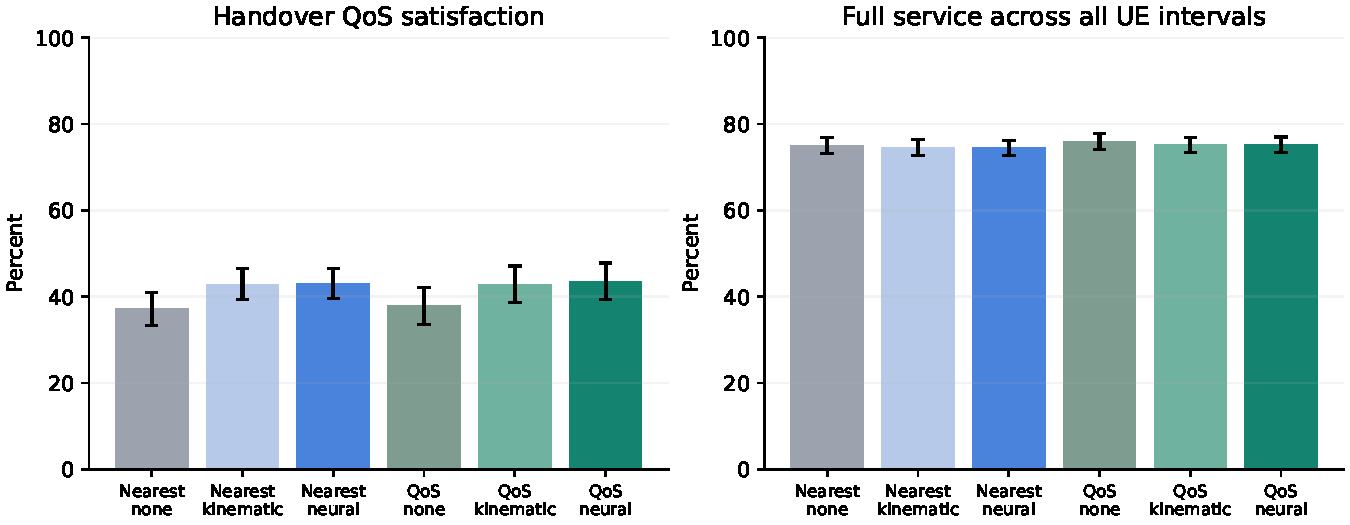
\includegraphics[width=.95\textwidth]{results/research_validation/event_and_network_service.pdf}
\caption{Event QoS and service over all UE intervals answer different questions. Error bars are 95\% intervals of the run-level mean, not paired comparison intervals.}
\end{figure*}

At four intervals, neural position RMSE is \NNPositionFour\ world units, versus \CVPositionFour\ for unperturbed constant velocity. At eight intervals the corresponding values are \NNPositionEight\ and \CVPositionEight. Neural demand MAE at eight intervals is \NNDemandEight\ RBs, versus \PersistDemandEight\ for persistence. These results do not support uniform positional superiority at every lead. Lead-one demand error is omitted from the demand-error plot because current demand is already observed.

\begin{figure*}[t]
\centering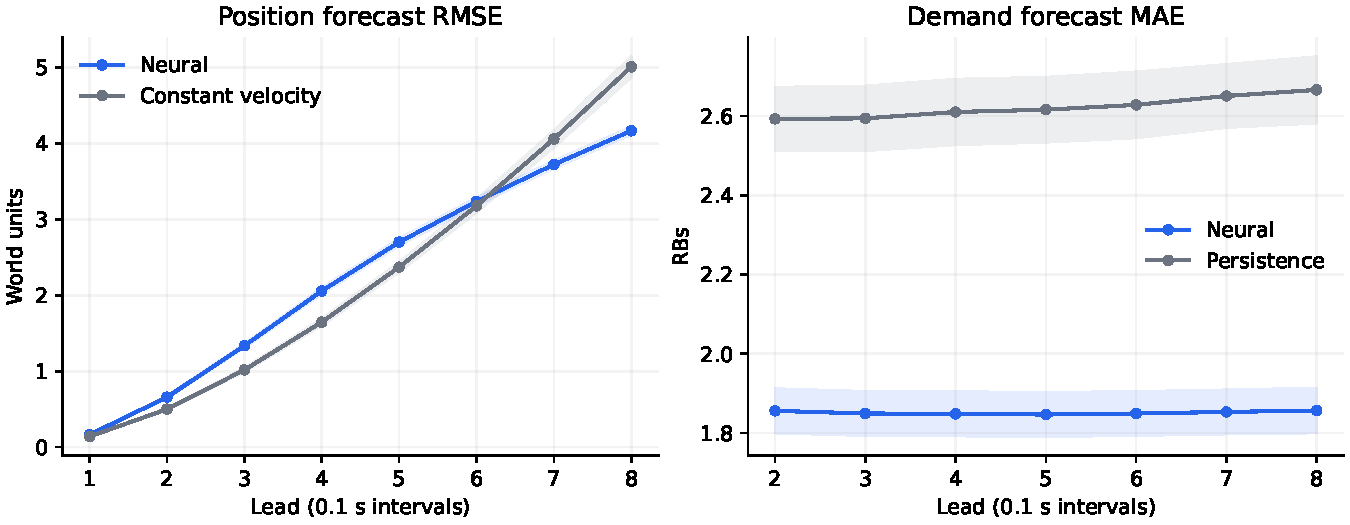
\includegraphics[width=.95\textwidth]{results/research_validation/forecast_comparison.pdf}
\caption{Forecast errors on held-out trajectories, aggregated first within each seed and then across 20 seeds. Shading gives 95\% intervals for mean error.}
\end{figure*}

Three additional predeclared initializations, 74--76, use the same training trajectories, validation trajectories, 30-epoch procedure, and all 20 test seeds. Their checkpoints and every test-run metric are retained under \texttt{results/training\_variability}. The primary live model remains initialization 73. The supplementary runs must be reported together rather than selecting the best test result. They examine initialization variability, not independence from the chosen synthetic workload.

\section{Reproduction and Limits}
The independent validation commands are \texttt{python -m proran.research\_validation}, \texttt{python -m proran.research\_report}, and \texttt{python -m proran.training\_variability}. The report records model and source SHA-256 hashes, Python/NumPy versions, configuration, raw run summaries, per-slice/per-lead forecast errors, and confidence intervals. It refuses to certify a run if simulator source changes during evaluation. Browser regression suites verify association links, interpolated movement, zoom behavior, slice-color ledgers, signal badges, all controller modes, responsive layout, and pause/replay behavior.

This study does not measure packet loss, physical spectral efficiency, HARQ, beam management, interruption duration, or 3GPP-compliant handover signaling. Rectangular training trajectories and small hexagonal UI demonstrations have different geometry and population/load distributions; their displayed metrics are not the paper's held-out workload. The synthetic periodic phase is observable in the forecast inputs and should not be assumed to exist in an operational network. Strict priority may disadvantage mMTC and is a declared scheduler assumption rather than an optimal fairness policy. Future work should use calibrated propagation and packet-level simulation, independent workloads, wider training replications, and learned target/action policies if those are the intended contributions.
\end{document}
